\chapter{Chefoo}

\begin{figure}[htbp]
\centering
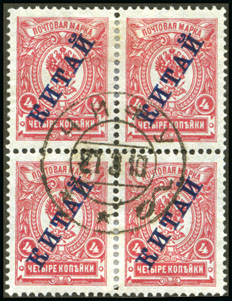
\includegraphics[width=.40\textwidth]{../russian-post-offices-in-china/10093.jpg}
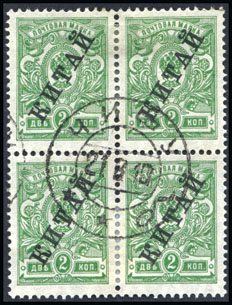
\includegraphics[width=.40\textwidth]{../russian-post-offices-in-china/10093-1.jpg}
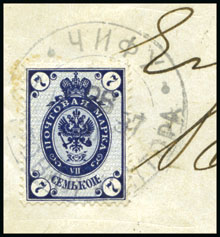
\includegraphics[width=.40\textwidth]{../russian-post-offices-in-china/10093-2.jpg}
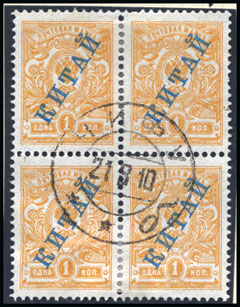
\includegraphics[width=.40\textwidth]{../russian-post-offices-in-china/10093-3.jpg}
\caption{
10093 CHEFOO: Selection of stamps cancelled in Chefoo incl. Arms 7k blue
tied on piece by 26.7.97 type 1 cds (earliest date known and illustrated
in "Stamps of the Russian Empire Used Abroad" p.340, ex R. S. Blomfield),
and 1910-16 "KITAI" 1k, 2k and 4k in blocks of four with CTO 21.3.1910 type 3B cds
\euro100.00 
}  
\end{figure} 

\begin{figure}[htbp]
\centering
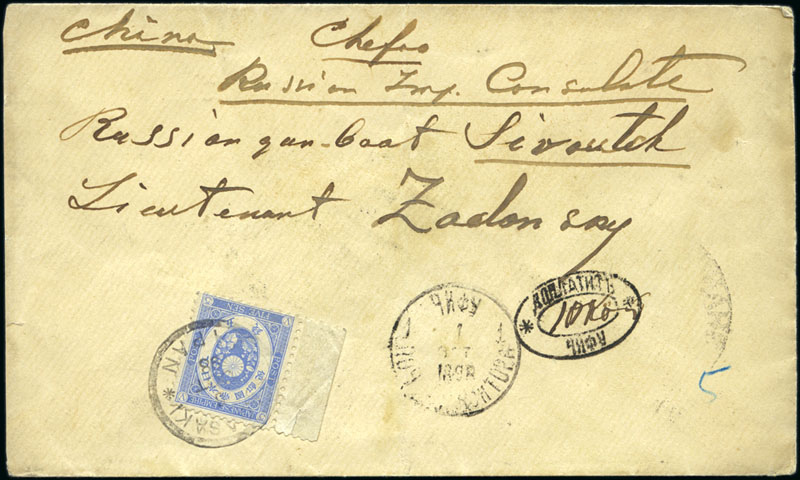
\includegraphics[width=.95\textwidth]{../russian-post-offices-in-china/10094.jpg}
\caption{
10094	CHEFOO INCOMING: 1898 Cover from Japan to the Russian Consulate in Chefoo,
for an Officer on a Russian gunboat, franked with 5s Koban tied by Nagasaki cds,
with transits of the Japanese P.O. at Shanghai and Chinese P.O. at Shanghai
and Chefoo on the reverse, and obverse with Chefoo Russian P.O. 1.10.98 arrival
cds (T\&S type 2) and oval tax hs "DOPLATIT / CHEFOO" with ms "10k", a rare
item of incoming mail with this tax mark
\euro 800.00 
}  
\end{figure} 

\begin{figure}[htbp]
\centering
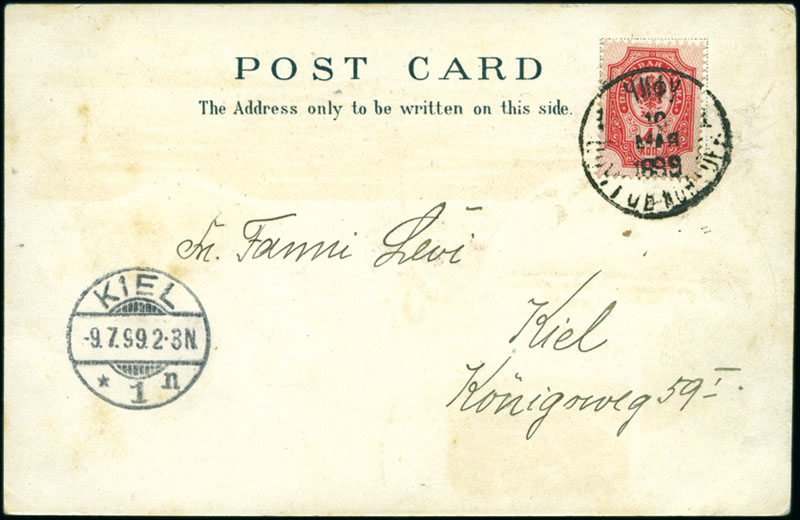
\includegraphics[width=.95\textwidth]{../russian-post-offices-in-china/10095.jpg}
\caption{
10095 CHEFOO: 1899 Picture postcard (with view of Chefoo port) sent to Germany
with ordinary Russia 4k tied by Chefoo 10.05.99 cds (T\&S type 2), 
Kiel arrival adjacent, a scarce usage of the postcard rate.

Note: Ordinary Russian stamps were only supplied to the Russian P.O. in Chefoo
up to 1899.
\euro400.00 
}  
\end{figure} 

\begin{figure}[htbp]
\centering
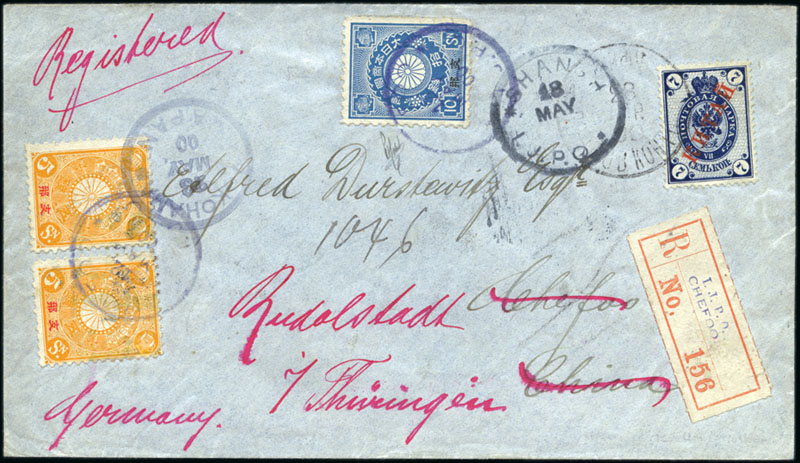
\includegraphics[width=.95\textwidth]{../russian-post-offices-in-china/10096.jpg}
\caption{
10096	CHEFOO: 1900 Cover sent locally in Chefoo with "KITAI" 7k, tied by 
Chefoo 28.4.00 cds (T\&S type 2), then re-addressed and sent registered to 
Germany from the Japanese P.O. at Chefoo and additionally franked with 5s (2) 
and 10s with Japanese China ovpts, "I.J.P.O / CHEFOO" registered label, 
with Shanghai Japanese P.O., Yokohama and Rudolstadt transits, a rare 
and attractive franking showing two different foreign P.O.s in Chefoo
\euro 500.00 
}  
\end{figure} 

\begin{figure}[htbp]
\centering
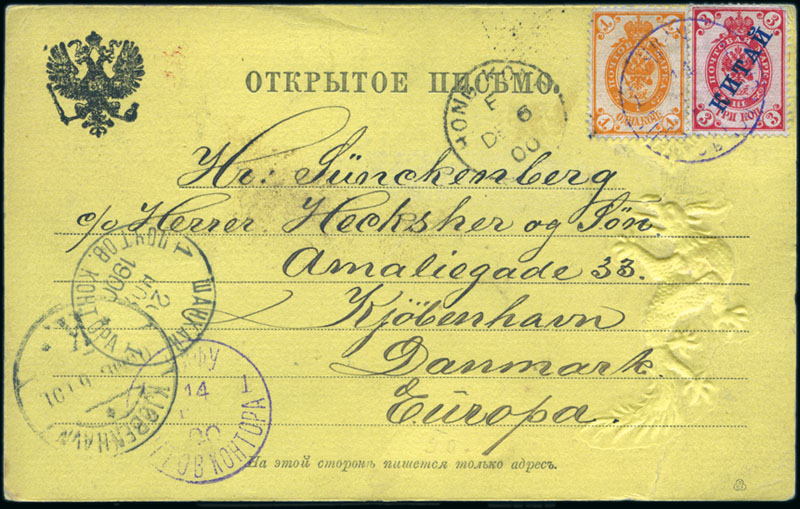
\includegraphics[width=.95\textwidth]{../russian-post-offices-in-china/10097.jpg}
\caption{
10097	CHEFOO: 1900 Decorative postcard (with gilt Chinese dragon and Imperial Eagle)
to Denmark, written on board SS "Normania" while in Talien Bay, franked 
with ordinary Russia 1k and "KITAI" 3k, reverse with Port Arthur 12.11.00 
cds (T\&S type 2D), put on a ship crossing the Strait of Pohai with stamps
tied on arrival by Chefoo 14.11.00 cds in violet (T\&S type 2), sent via the
Chinese P.O. at Chefoo and Shanghai, then via Hong Kong and finally Copenhagen, 
an attractive
\euro 500.00 
}  
\end{figure} 

\begin{figure}[htbp]
\centering
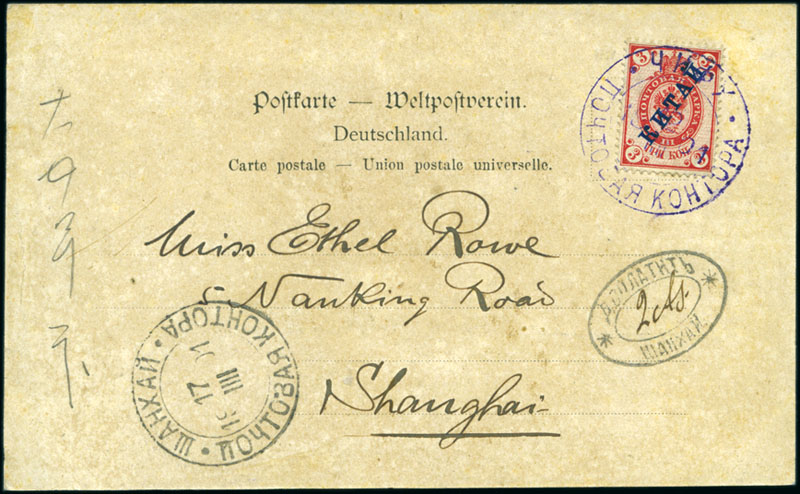
\includegraphics[width=.95\textwidth]{../russian-post-offices-in-china/10098.jpg}
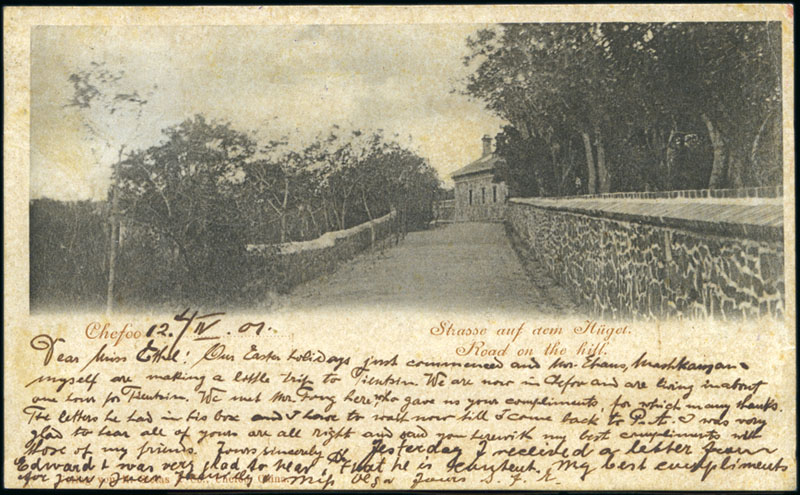
\includegraphics[width=.95\textwidth]{../russian-post-offices-in-china/10098-1.jpg}
\caption{
10098	CHEFOO: 1901 Postcard to Shanghai with "KITAI" 3k tied by Chefoo 
12.IIII.01 cds in violet (T\&S type 1), with Shanghai Russian 
P.O. 17.IIII.01 arrival (T\&S type 1) and oval "DOPLATIT / SHANGHAI" 
tax mark with ms "2c" (not recorded by T\&S), very rare
\euro 600.00 
}  
\end{figure} 

\begin{figure}[htbp]
\centering
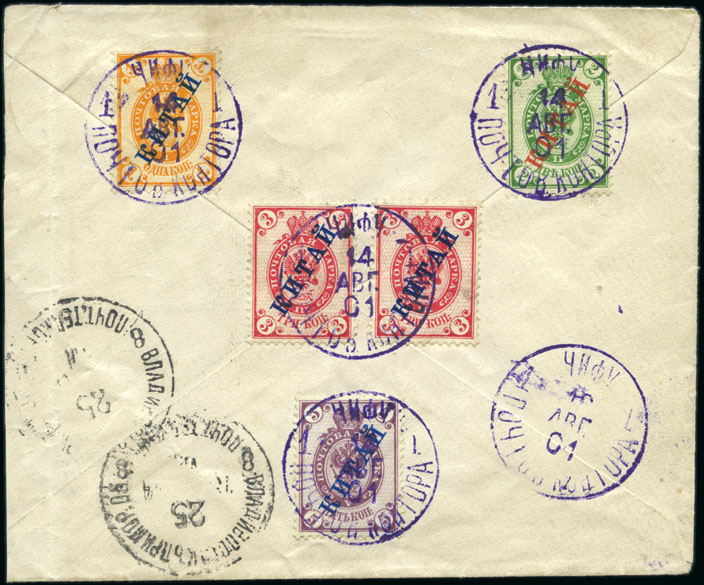
\includegraphics[width=.95\textwidth]{../russian-post-offices-in-china/10099.jpg}
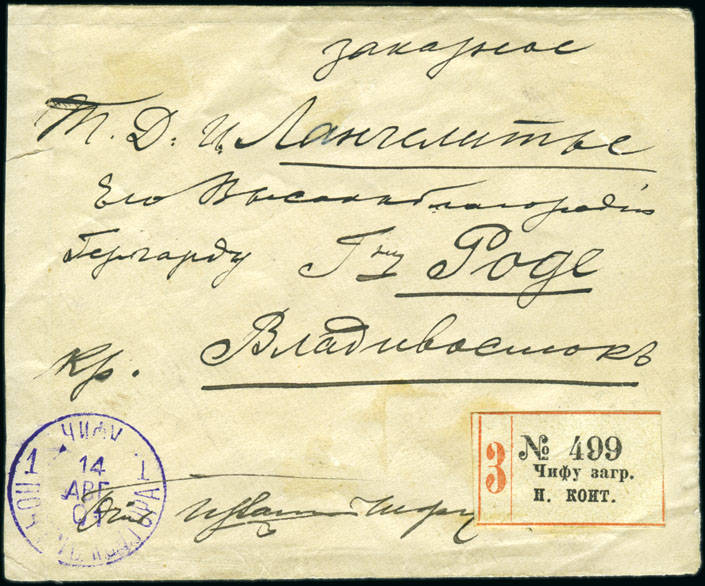
\includegraphics[width=.95\textwidth]{../russian-post-offices-in-china/10099-1.jpg}
\caption{
10099	CHEFOO: 1901 Cover to Vladivostok franked on reverse with "KITAI" 1k, 
2k, 3k (2) and 5k, all tied by Chefoo 14.08.01 cds in violet (T\&S type 2), 
obverse with "Chefoo / Post Office Abroad" registration label in Cyrillic, 
Vladivostok bs, opened for display, attractive and colourful franking
\euro 500.00 
}  
\end{figure} 













  
  
  
  
  
  
  
  
  
  
  
  
  
  
  
    